\section{Development process}
\label{sec:DevelopmentProcess}

\subsection{Agenda consultation}
The IASB conducts a comprehensive review of its technical agenda every three years, although, of course, it stands ready to address urgent issues rapidly if the need arises. On the basis of public input received during the triennial agenda consultation, the IASB develops a three- to  five-year agenda of projects. Apart from the reviews, the IASB and/or the Interpretations Committee evaluate all requests received for possible interpretation or amendment of a Standard.

\subsection{Research programme}
Once a project has been identified as a candidate for a possible Standard, the IASB staff undertake a programme of research aimed at gathering evidence to de ne the problem and identify whether there is a  financial reporting matter that justifies an effort by the IASB.
The evidence-gathering includes (for major projects) soliciting public input via a Discussion Paper or similar document. National accounting standard-setters are invited to help in the research effort. The research programme leads either to a project proposal or to a recommendation not to develop a Standard.

\subsection{Standards programme}
If the IASB decides to develop a Standard, it reviews the results of the research, including the comments received on the Discussion Paper, and develops proposed solutions to the issues that were identified. To assist
in developing the proposed solutions, the IASB often appoints a working group of experts on the issue. It also consults with the Advisory Council and the ASAF. The IASB publishes its proposals in the form of an Exposure Draft. Public comments are invited. To gather additional evidence, IASB members and staff undertake worldwide outreach by various means, including round-table meetings and webcasts, with special efforts to obtain the views of users of  financial statements. The culmination of the standards programme is the issue of a new or amended Standard.

\subsection{Implementation}
The IASB monitors the implementation of new or amended Standards to identify any implementation problems that may need to be addressed by an Interpretation or a narrow-scope amendment to the Standard.
The Interpretations Committee takes the lead in developing the Interpretations or amendments for  final clearance by the IASB. Public comments are invited. Once a new Standard or major amendment has been in place for several years, the IASB conducts a Post-implementation Review to assess whether the Standard is achieving its objective and, if not, what amendments should be considered.

\subsection{Summary}
\begin{figure}[h]
\caption{Development process summary}
\centering
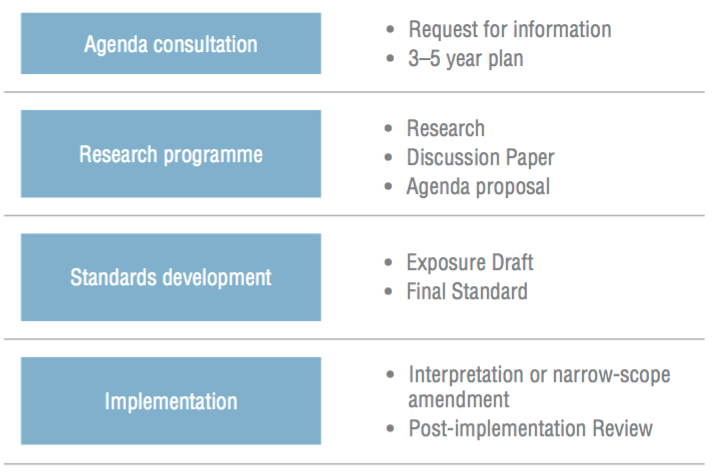
\includegraphics[width=0.8\textwidth]{images/devprocess.png}
\end{figure}